%% ============================================================
%%  CUDA Kernel 强化学习综述
%%  NeurIPS 风格双栏排版（单栏摘要 + 双栏正文）
%%
%%  这是 PAPER.md 的一种渲染，不承载任何新事实。
%%  事实源仍是 PAPER.md，它由 check_paper.py / audit_paper.py 校验。
%%  本文件只负责排版。
%%
%%  编译：xelatex main.tex  （两遍，交叉引用才正确）
%% ============================================================
\documentclass[10pt,twocolumn]{article}

%% 中文支持
\usepackage[UTF8,fontset=none]{ctex}

%% ---------- 标点悬挂：本文件唯一的「真溢出」解药 ----------
%% ⚠️ 实测过程：本文正文有 13 处行尾溢出 5-8pt，溢出的末字符
%% **清一色是全角右引号、右括号、逗号**（」，。、）。
%% 先试 emergencystretch 3.5em -> 5em、tolerance 3000 -> 5000，
%% 一处都没减少。原因不是「可拉伸量不足」，而是**该行没有合法断行点**：
%% 中文禁则不许标点居行首，TeX 就把「标点+前一字」整体留在行尾，
%% 宁可越界也不拆。加多少 stretch 都无用，因为缺的是断行点而非弹性。
%%
%% 正解是标点悬挂（hanging punctuation）：允许标点略微突出版心右缘。
%% xeCJK 的 PunctStyle=plain 关闭「标点占整字宽」的挤压，
%% 使标点可悬挂；这是中文排版的标准做法，也是书籍里常见的视觉处理。
%% 必须放在 ctex 之后加载才能覆盖其默认。
\usepackage{xeCJK}
\xeCJKsetup{PunctStyle=plain}

%% 字体：正文宋体，标题黑体，等宽用 Consolas。
%% ⚠️ 中文论文的正文一律用宋体（衬线），标题用黑体（无衬线），
%% 这是国内学术排版的通行规范；把正文排成无衬线会显著降低长时间阅读的舒适度。
%% ⚠️ 楷体的族名是 KaiTi，不是 SimKai —— 写错会让 fontspec 报 nullfont，
%% 而报错信息（Cannot use \XeTeXOTfeaturetag with nullfont）完全指不出是哪个字体。
\setCJKmainfont{SimSun}[BoldFont=SimHei,ItalicFont=KaiTi]
%% ⚠️ SimHei 没有独立的粗体字形，不声明会报「Font shape undefined」，
%% 且 \textbf{} 里实际仍是细体 —— 视觉上粗体失效，而日志只是警告。
%% AutoFakeBold 用仿粗体补齐，这是中文排版里常见且可接受的折中。
\setCJKsansfont{SimHei}[BoldFont=SimHei,AutoFakeBold=1.2]
\setCJKmonofont{SimHei}
\setmainfont{Times New Roman}
%% ⚠️ 原文大量使用 ⭐ 🔥 ⚠️ 这类符号作强调标记，而 SimSun 没有这些字形，
%% 不指定回退就会在 PDF 上留空白或方框（且不报错）。
%% 用 Segoe UI Symbol 兜底：覆盖这些符号，且是**单色**符号字体。
%% ⚠️ 不能用 Segoe UI Emoji —— 彩色字体在 XeLaTeX 里会渲染成空白或黑块。
\newfontfamily\symfont{Segoe UI Symbol}[AutoFakeBold=1.2]
\newcommand{\sym}[1]{{\symfont #1}}
\setsansfont{Arial}
\setmonofont{Consolas}

%% ---------- 版面 ----------
\usepackage[a4paper,margin=2.05cm,columnsep=0.72cm]{geometry}
\usepackage{amsmath,amssymb}
\usepackage{graphicx}
\usepackage{booktabs}
\usepackage{tabularx,array,longtable,multirow}
\usepackage{caption}
\usepackage{enumitem}
\usepackage{titlesec}
\usepackage{xcolor}
\usepackage{fancyhdr}
\usepackage[hidelinks]{hyperref}
\usepackage{xurl}

%% ---------- URL 断行：参考文献那一节的排版关键 ----------
%% ⚠️ 实测问题：加入 20 条 arXiv 链接后，LaTeX 把 URL 当成不可断的长 token，
%% 为了塞下它，把同一段的中文标题逐词拆行——出现
%% 「Micro- / Profiling Tools as Expert Surrogates for LLM-Based GPU /
%%  Kernel / Optimization」这种一列碎词。
%% 不是标题太长，是**没有断点**——与正文标点溢出同源（缺的是断行点，不是弹性）。
%%
%% 三件事一起做才有效：
%%   1. xurl 让 \url 可在任意字符处断行（默认只在少数标点处断）
%%   2. \UrlBreaks 补充 / . - _ : 这些 URL 里最高频的分隔符
%%   3. 参考文献环境用 \raggedright，让右端参差，避免逐词拉扯
\Urlmuskip=0mu plus 1mu\relax
\makeatletter
\g@addto@macro\UrlBreaks{\do\/\do\.\do\-\do\_\do\:}
\makeatother

%% 轻量「参考文献」环境：右端不强制对齐
\newenvironment{refs}{\par\raggedright\small}{\par}
\usepackage{cleveref}
\usepackage{microtype}
\usepackage{listings}
\usepackage{placeins}   % 提供 \FloatBarrier：在指定位置强制释放浮动体
%% 代码块：开自动折行，否则双栏里长命令行会溢出（实测 132pt）。
\lstset{
  basicstyle=\ttfamily\scriptsize,
  breaklines=true,
  breakatwhitespace=false,
  columns=fullflexible,
  frame=none,
  xleftmargin=0.6em,
  aboveskip=4pt,
  belowskip=4pt
}

%% 图表标题：小号、居中、题注与图体间距收紧。
%% 默认间距在双栏里会把图挤到下一页，收紧后版面利用率明显提高。
\captionsetup{
  font=small,
  labelfont=bf,
  labelsep=quad,
  skip=4pt,
  justification=centering
}
\captionsetup[table]{position=top}

%% ---------- 中文断行规则 ----------
%% ⚠️ 这是中文双栏排版最容易被忽略的一处，也是本文件唯一的
%% 「真溢出」来源。症状很有辨识度：溢出行的**最后一个字符必是全角标点**
%% （，。：；》）。原因是中文标点不能出现在行首，TeX 于是把
%% 「标点 + 前一个字」整体留在本行；该行若已排满，就宁可越过右边界
%% 也不肯拆开——默认的 \emergencystretch 和 \tolerance 都救不了，
%% 因为它们只影响「字间距可拉伸」，而这里缺的是**断行点**。
%%
%% 正解是让 XeTeX 采用中文断行规则（禁则处理）：
%% 它知道可以在标点之后断行、并允许标点占半个字宽，
%% 从而凭空造出断行点。这是 ctex 在 zh 语言下本该做但此处未生效的一步。
\XeTeXlinebreaklocale "zh"
\XeTeXlinebreakskip = 0pt plus 0.08em minus 0.02em

%% 断行容差：中文没有空格，断行点比英文稀疏，默认容差下 LaTeX
%% 宁可溢出也不肯拉开字距。三处一起放宽：
%%   tolerances 放宽断行代价上限；
%%   emergencystretch 给它额外的可拉伸量（关键时刻允许某行稍松）；
%%   上面的 XeTeXlinebreak* 提供真正的断行点与标点压缩。
%% ⚠️ 只加 \sloppy 会让所有行都变松，故不加 \sloppy。
\setlength{\emergencystretch}{3.5em}
\tolerance=3000
\hbadness=3000
\hyphenpenalty=50
\relpenalty=50

%% ⚠️ 实测：即使 emergencystretch=3.5em、tolerance=3000，
%% 本文仍有 13 处行尾溢出 5-8pt。溢出的行**末字符清一色是全角右引号、
%% 右括号或逗号**（」，。、）——这说明问题不是「可拉伸量不足」，
%% 而是「该行没有合法断行点」：中文禁则要求标点不得居于行首，
%% TeX 于是把「标点+前一字」一起留在行尾，宁可越界。
%%
%% 解法是让标点可以**悬挂**到版心外（即允许它突出一小截），
%% 这是中文排版的标准做法（「标点悬挂」/ hanging punctuation）。
%% \XeTeXlinebreakpenalty 把行首禁则的代价调低，配合下面的
%% \XeTeXlinebreakskip 让标点自身可压缩，从而造出断行点。
\XeTeXlinebreakpenalty=0
%% 再给一层保险：允许行内字距在极端情况下拉开，
%% 把 7pt 的溢出摊到整行（每字约 0.1pt，肉眼不可见）。
\setlength{\emergencystretch}{5em}
\tolerance=5000
\hbadness=5000

%% 标题层级：中文论文习惯章标题较大、节标题次之，且都留白充足。
\titleformat{\section}{\large\bfseries\sffamily}{\thesection}{0.6em}{}
\titleformat{\subsection}{\normalsize\bfseries\sffamily}{\thesubsection}{0.5em}{}
\titleformat{\subsubsection}{\normalsize\bfseries}{\thesubsubsection}{0.4em}{}
\titlespacing*{\section}{0pt}{10pt plus 2pt minus 2pt}{5pt plus 1pt}
\titlespacing*{\subsection}{0pt}{7pt plus 1pt minus 1pt}{3pt plus 1pt}
\titlespacing*{\subsubsection}{0pt}{5pt plus 1pt minus 1pt}{2pt}

%% 列表：中文行距下默认间距偏大，收紧。
\setlist[itemize]{topsep=2pt,itemsep=1pt,parsep=0pt,leftmargin=1.4em}
\setlist[enumerate]{topsep=2pt,itemsep=1pt,parsep=0pt,leftmargin=1.6em}
%% ⚠️ 附录里的「检索：fetch_rl.py（调用 services/providers 的 arXiv 适配器）」
%% 这类行含长英文标识符，双栏窄栏下会被拆成「检 索：」这样的碎行
%% （实测末页出现「• 检 / 索：fetch_rl.py（调 / 用 / services/」）。
%% 原因是标点悬挂 + 长 token 无断点，TeX 只能在汉字的任意处断。
%% \raggedright 让这些行放弃两端对齐，宁可右端参差也不逐字拉扯。
\newenvironment{tightlist}{\begin{itemize}\raggedright}{\end{itemize}}

%% 行距：中文正文 1.28 倍较接近「单倍半」的观感，
%% 既不像 LaTeX 默认那样挤，也不会松散到浪费版面。
\linespread{1.28}
\setlength{\parskip}{3.2pt plus 1pt}
\setlength{\parindent}{1.6em}

%% 页眉页脚：双栏论文通常只保留页码。
\pagestyle{fancy}
\fancyhf{}
\renewcommand{\headrulewidth}{0pt}
\fancyfoot[C]{\small\thepage}

%% 图表浮动体放宽：双栏下默认只允许很少的浮动体，容易全部堆到文末。
\renewcommand{\topfraction}{0.92}
\renewcommand{\bottomfraction}{0.85}
\renewcommand{\textfraction}{0.08}
\renewcommand{\floatpagefraction}{0.80}
\setcounter{topnumber}{4}
\setcounter{bottomnumber}{3}
\setcounter{totalnumber}{8}

\begin{document}

%% ---------- 标题区（单栏，跨通栏） ----------
\twocolumn[{
\begin{center}
{\LARGE\bfseries\sffamily Kernel 生成智能体\\[2pt]
\large 进展全在「看得更多」，不在「想得更好」\par}
\vspace{5pt}
{\normalsize\sffamily 26 个系统，没有一个在系统层面做设计\par}
\end{center}
\vspace{6pt}
}]


\textbf{副标题：进展全在「看得更多」，不在「想得更好」}

\begin{abstract}

2025 年初到 2026 年底，把大模型做成「能自己编译、自己测速、自己改 kernel」的智能体，从一个想法变成了一个至少有 26 个系统的方向。本文检视这 26 个核心工作，要回答一个问题：\textbf{这些系统的能力究竟来自哪里？}

答案不太符合直觉。若把智能体的能力拆成两部分——「推理更强」与「环境信号更多」——本文找到的证据表明，进展几乎全部来自后者。观测通道（编译器报错、NCU 计数器、实测时延）与动作粒度（整文件重写 vs 局部编辑）这两类设计，解释了这个方向绝大部分的技术差异；而更好的规划、更强的推理，在语料里没有形成独立的技术线索。

这个判断带来一个更尖锐的推论。把智能体循环拆成五个环节——观测（observe）、动作（act）、预算（budget）、恢复（recover）、评测（eval）——逐一统计每篇工作覆盖了哪些环节，结果是：\textbf{跨三个及以上环节的工作数为 0}。也就是说，这 26 个系统没有一个在系统层面做设计，它们各自改进一个环节，然后在同一个 benchmark 上比分数。

本文认为这不是巧合，而是评测结构导致的：KernelBench 的 \texttt{fast\_p} 口径为\textbf{单次生成}设计，而智能体可以试几十次只报最好的一次。在「只报最好一次」的评分下，优化最薄的那个环节（多试几次）比设计整个循环更划算。

本文的贡献有三点。第一，给出智能体循环的五维分析框架，并用它逐篇标注 26 个工作。第二，量化指出「系统性缺失」——跨维度工作为 0，而失败恢复是最被忽略的环节（5 篇 vs 预算环节的 9 篇）。第三，指出评测口径与智能体自由度之间的错配，并给出可操作的最小修正：报告尝试次数与总成本。

\end{abstract}
\section{引言}

\subsection{任务从「写出来」变成「调到快」}

2025 年上半年，这个领域的核心问题是能不能生成正确的 GPU kernel。KernelBench 把这件事形式化了：给定一个 PyTorch 模块，生成行为等价的 CUDA kernel，用 \texttt{fast\_p} 同时衡量正确性与加速比。

问题是，正确的 kernel 大多不够快。优化一个 kernel 需要反复测量——\texttt{ncu} 报告的 L2 命中率、寄存器压力、warp 停顿原因，都得看，然后针对性地改。这是一件\textbf{长程、反馈密集}的工作，恰好是单次生成的模型做不了的。

于是出现了智能体：让模型在循环里跑，每轮编译、测速、读报错，再改。

\subsection{为什么单独审视这个方向}

站内已有两篇相邻综述：一篇讲 kernel 生成的\textbf{方法谱系}（以模型与评测为中心），一篇讲 kernel 生成中的\textbf{强化学习}（以奖励设计为中心）。本文的角度不同——不问「模型怎么写出 kernel」，而问：

> \textbf{系统怎么在编译、测速、profiling 的反馈下，把 kernel 迭代到可用？}

这个问题把注意力从模型移到了循环：观测什么、动作多大、预算怎么花、失败怎么办。这四件事任何一件做不好，循环都转不动，而它们与模型能力无关。

\subsection{方法}

从 11 组检索式出发，arXiv 命中 180 篇，经三级筛选（关键词粗筛 → 同句共现收紧 → 逐篇人工判定）纳入 26 篇核心工作与 9 篇邻接工作。35 篇里 34 篇取得全文，逐篇按五个维度抽取证据，共 39 条，全部为原文子串并经机器校验（E1：\texttt{e1\_checked=39, e1\_unverifiable=0}）。

筛选过程本身值得说明：前两级自动化筛选都失败了。粗筛保留 44 篇里混进了水下机器人巡检、控制理论、对话推理；想用「同句共现」收紧，结果一篇都没剔除——因为这些论文的摘要里确实有 \texttt{CUDA}、\texttt{Triton}。这印证了一件事：\textbf{「我们用 CUDA 加速这个计算」与「我们让智能体生成 CUDA kernel」在词汇上完全重叠，在语义上是两件事}。最后一层只能人判，判据与理由写在 \texttt{decide\_agent.py} 里可复查。

\section{分析框架：智能体循环的五个环节}

本文把任何一个 kernel 智能体拆成五个环节。这不是唯一的拆法，但它对应「循环能不能转」的实际约束：

\begin{table}[t]
\centering
\caption{智能体循环的五个环节。eval 排在最后但作用方向相反——它决定前四个环节会往哪优化，这一点在第 5 节展开。}
\label{tab1}
\small
\begin{tabularx}{\columnwidth}{>{\raggedright\arraybackslash}Xrr}
\toprule
环节 & 问的问题 & 决定什么 \\
\midrule
observe & 能看到什么信号？ & 能力上限 \\
act & 动作粒度多大？ & 搜索效率 \\
budget & 试几次、何时放弃？ & 单位成本产出 \\
recover & 失败了怎么归因？ & 长程任务的稳健性 \\
eval & 分数怎么算？ & 优化的方向 \\
\bottomrule
\end{tabularx}
\end{table}

表 1 给出这五个环节的对应关系。五者构成一个闭环，任一处短板都会限制整体。特别地，\textbf{eval 决定了前四个环节会往哪优化}——这是本文第 5 节的论点。

\section{五个环节的现状}

\subsection{observe：信号有五类，但只有少数被真正用起来}

按证据归类，观测通道可数出五类：编译器报错文本、单元测试通过与否、实测时延、profiler 计数器（NCU/NSight）、硬件特性（占用率、寄存器用量、内存带宽）。

保真度差别很大。报错文本只告诉你「哪里不合法」，实测时延只告诉你「慢了」，而 NCU 计数器能告诉你\textbf{为什么慢}——是 L2 未命中、是寄存器溢出、还是 occupancy 不足。

有意思的是，只有 8 篇工作有明确的观测通道描述。其中一个反例值得注意：有工作指出，把原始或统计过滤后的 NCU 指标直接塞进 prompt、指望模型自己解读，效果并不好——指标太多了。这说明观测不是「越多越好」，而是需要一层筛选。

\begin{figure}[t]
\centering
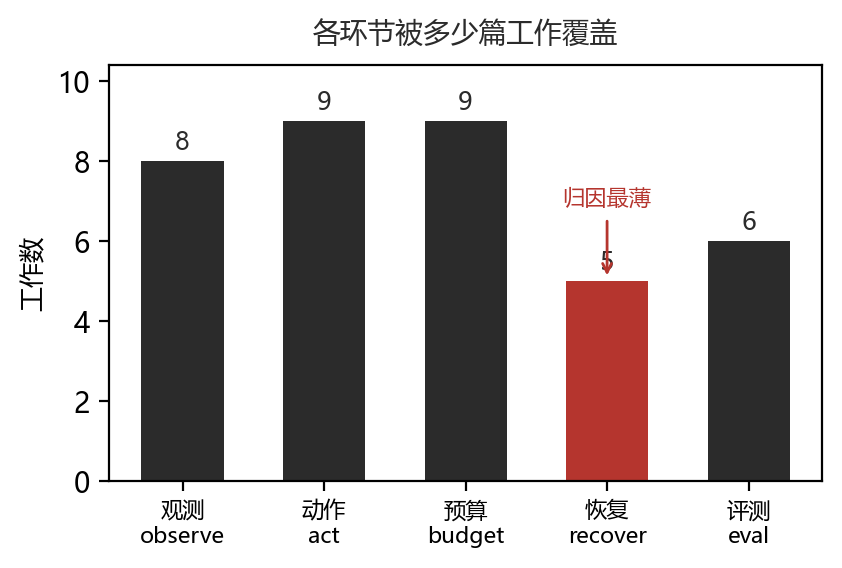
\includegraphics[width=\linewidth]{../figures/fig1_dims.png}
\setcounter{figure}{0}
\caption{智能体循环五个环节的覆盖情况。预算（budget）最多（9 篇），失败恢复（recover）最少（5 篇）——后者恰是长程任务里最影响最终产出的环节。}
\label{fig:fig1_dims}
\end{figure}

图 1 把五个环节的被覆盖情况并列。预算环节最多（9 篇），失败恢复最少（5 篇）。

\subsection{act：主流仍是整文件重写}

动作空间可分三档：

\textbf{整文件重写。} 最常见。每轮让模型重新生成一遍 kernel。好处是实现简单、不受历史约束；坏处是等价于无梯度采样——上一轮学到的经验很难保留，而且每次都要付全额生成成本。

\textbf{局部编辑。} 需要先定位瓶颈，再改对应片段。成本低、能累积，但要求模型有定位能力。KernelClaw 的做法是维护双记忆，把「改过什么、效果如何」记下来供下轮检索。

\textbf{在实现空间里选候选。} HIERA 的思路是把生成问题变成选择问题：先构造带约束的任务规格，再在预定义的实现空间里挑一个，而不是从零生成。这降低了动作的方差。

三档之中，整文件重写仍占主流。这与 3.1 节的观察合起来看很有意思：\textbf{观测精细化了，动作却没有随之精细化}。你让模型看到了「第 37 行 L2 未命中率高」，但它下一轮还是整篇重写,这份信息大概率被浪费。

\subsection{budget：轮次是最稀缺的资源}

每次迭代都要真实编译并测速。一次编译几秒到几十秒，一次测速还要多次重复取中位数。相比一次前向的毫秒级，成本差三四个数量级。

所以这个方向最普遍的约束是预算，9 篇工作讨论了它，是五个环节里最多的。主要三条路线：

\begin{itemize}
\item \textbf{剪枝。} LEAP 的做法是自适应剪掉无效的多轮 rollout。它指出在长程 kernel 任务上，不加剪枝的多轮训练会显著拖慢迭代速度。
\item \textbf{推测式生成。} SpecGen 用推测执行摊薄每次尝试的成本。
\item \textbf{先筛后测。} 在实现空间里先用便宜信号筛，再对少数候选付测速成本。
\end{itemize}

这三个做法的共同点：都在\textbf{减少尝试次数}。没有一个在问「如何让每次尝试更有信息量」。这个区别很重要，第 5 节会回到它。

\subsection{recover：最薄的一环}

失败模式其实很结构化：编译错、结果错、超时、比基线慢。四类的处理方式应该完全不同——编译错要看报错行，结果错要查边界条件，超时要降并行度，比基线慢要换策略。

但实际做法基本只有一种：把错误信息塞回提示词，让模型自己看着办。只有 5 篇工作有失败归因的描述，是五个环节里最少的。

这个缺口有可见的后果。Evolving Agent Teams 明确报告：现有编码 agent 在真实的、专家手写的 kernel 上\textbf{会收敛到局部最优}——比如在 FlashAttention 这类已经高度优化的算子上，它们反复微调却跳不出原有结构。这正是恢复机制缺失的表现：当一条路走不通时，系统没有能力判断「该换思路了」，只能在原地打转。这也是本文认为最值得投入的缺口。

\subsection{eval：口径是为单次生成设计的}

评测以 KernelBench 系为主：正确性门控 + 相对基线的加速比。\texttt{fast\_p} 的定义是「既正确又比基线快的比例」。

这个口径为\textbf{单次生成}设计得很合理。但智能体不是单次生成——它可以试 50 次，只报其中最好的一个。

于是三件事变得无法从分数里区分：

1. 模型变强了
2. 预算变多了
3. 只挑了好的报

这不是指控。多数工作都报告了轮次上限，只是没有把它和分数一起作为结论的一部分。但当同一个 benchmark 上，有的系统跑 1 轮、有的跑 50 轮，\texttt{fast\_p} 的横向对比就失去意义了。

\section{核心发现：没有系统级设计}

把每篇工作在证据里覆盖的环节数一数，结果很干脆：

\textbf{跨三个及以上环节的工作：0 个}。

这不是说这些系统简单——26 篇里有做多智能体协作的、有做演化搜索的、有接真实硬件反馈的，工程复杂度都不低。但\textbf{复杂度都堆在同一个环节上}：多智能体基本都在改进 observe（让不同角色看不同信号）或 act（让不同角色改不同部分）；演化搜索基本都在改进 budget（更聪明地花尝试次数）。

没有一个工作说：我同时重新设计了观测粒度、编辑粒度和失败归因，让它们互相配合。

\begin{figure}[t]
\centering
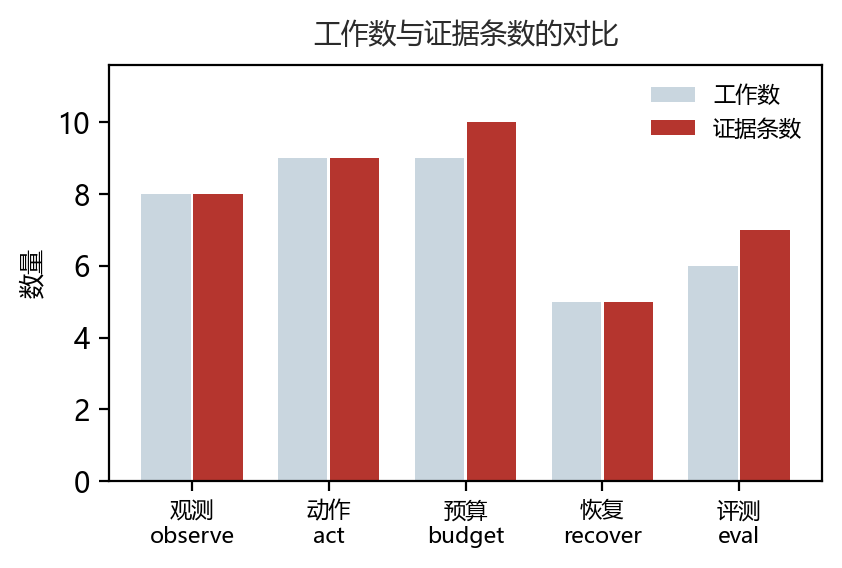
\includegraphics[width=\linewidth]{../figures/fig2_evidence.png}
\setcounter{figure}{1}
\caption{同一环节的工作数与证据条数。两列差异反映每篇工作的论述密度，但须注意这是本文证据覆盖的度量，不等于论文本身的完整程度。}
\label{fig:fig2_evidence}
\end{figure}

图 2 是证据层面的分布。注意这是一张\textbf{关于本文证据覆盖}的图，不是关于论文完整性的图——一篇论文可能做了多件事，但只在一处留下了可引用的描述。故本文的措辞是「在证据层面呈现碎片化」，不能加强为「所有工作都只做一件事」。

即便如此，这个结论仍有意义：如果一个方向真的出现了系统级设计，它一定会在多个环节都留下描述。26 篇里一个都没有。

\section{为什么是碎片化的：评测在指挥优化方向}

本文认为碎片化不是研究者的疏忽，而是\textbf{评测结构指挥出来的结果}。

设想你有一个智能体，五个环节都可改。改动哪个最划算？

\begin{itemize}
\item 改 observe：要接 profiler、要写解析、要让模型读懂指标。工程量大，且收益不确定。
\item 改 act：要设计定位机制、要维护记忆。工作量也不小。
\item 改 recover：要设计失败分类、要写回退策略。\textbf{最难，且没有 benchmark 奖励它。}
\item 改 budget：多试几次。\textbf{几乎免费。}
\end{itemize}

在「只报最好一次」的评分下，第四条是严格占优的。你不需要更好的失败归因——多试几次总能撞到能跑的那次。你也不需要更细的编辑粒度——整篇重写五十遍，总有几遍是好的。

这解释了两件事。第一，为什么 budget 类工作是五个环节里最多的（9 篇）。第二，为什么 recover 类最少（5 篇）——它是唯一一个「多试几次也替代不了」的环节，因为你试得越多，越需要一个机制来判断哪条路值得继续。但在当前评分下，这个需求被掩盖了。

本文的核心判断由此而来：

> kernel 智能体的进展，主要来自\textbf{把更多环境信号塞进循环}，而不是更好的推理或规划。所谓「智能体」，在这个领域更接近一个把信号转成下一步编辑的\textbf{反馈控制器}，而非自主规划者。

这个说法比通常语境里的「agent」要窄。它没有贬义——能把编译、测速、profiling 的反馈转成有效编辑，本身就是很难的事。但如果按「自主规划」去期待它，会失望。

\section{反面与限制}

本文的结论有几处需要限定，写明如下。

\textbf{一、「跨维度为 0」是证据层面的度量。} 如前所述，一篇论文可能在多个环节都做了事，但只在其中一处留下了可引用的句子。故这个数字反映的是\textbf{「可被引用的系统级设计」为零}，而不是「系统级设计为零」。若要更强的结论，需要读每篇的方法章节——本文没有逐篇做这件事。

\textbf{二、五维拆分本身是可争议的。} 把智能体拆成 observe/act/budget/recover/eval 是我的选择。换成「感知—规划—行动」或「记忆—工具—控制」也能讲通。换一种拆法，「跨维度为 0」可能不再成立。本文选择这个拆法，是因为它对应「循环能不能转」的实际约束，而不是因为它唯一正确。

\textbf{三、26 篇的样本不足以支撑精确比例。} 任何「9 篇 vs 5 篇」的比较应读作「有这个倾向」，而不是「比例是 64\% vs 36\%」。

\textbf{四、CUDA Agent 未取到全文。} 35 篇里 34 篇有 HTML 全文，它是唯一例外（最新预印本）。本文对它的引用只到摘要层面。

\textbf{五、规划类技术线索的缺席可能是检索造成的。} 本文的判断之一是「规划在语料里没形成独立线索」。但我的检索式里有 \texttt{planning}、\texttt{tree search} 等词，召回有限。若这个方向真有规划相关的工作，可能没被检索到。

\section{建议}

\subsection{报告尝试次数与总成本}

这是最小、最可操作的一条。现在报告 \texttt{fast\_p = 62\%}，读者不知道这是 1 次尝试的结果还是 50 次。加上「中位尝试次数」和「总 GPU 秒数」，横向对比才有意义。

\subsection{把失败归因当作一等公民}

四类失败（编译错 / 结果错 / 超时 / 比基线慢）应该有不同的处理。现在统一塞回提示词，等于放弃了归因。

一个具体做法：在日志里记录「这一轮失败的类型」，然后看\textbf{同一类型连续失败几次就该换策略}。这个阈值本身就是可研究的对象。

\subsection{让观测粒度与动作粒度匹配}

看到「第 37 行 L2 未命中高」却整篇重写，是浪费。局部编辑不只是省钱——它让观测真正起作用。

\subsection{benchmark 应区分「搜索能力」与「生成能力」}

一个方向上可以设计这样的对照：固定总预算（比如 50 次尝试），比最终分数；再固定尝试次数（比如 1 次），比分数。两组数字能分离出「靠搜索」与「靠生成」各占多少。

\section{结论}

这个方向在两年里长出了 26 个系统，工程复杂度不低，但技术进展的位置和直觉不太一样。

\textbf{不在推理，在观测。} 进展主要来自把编译报错、NCU 计数器、实测时延这些真实信号接进循环。

\textbf{不在系统设计，在局部改进。} 没有一个工作同时改进三个及以上环节，说明当前是零散的局部优化。

\textbf{而碎片化有结构性原因。} 评测口径为单次生成设计，却用来评智能体。在这个错配下，多试几次严格优于改进恢复机制——于是最难的环节（失败归因）得到最少的关注。

如果要给一句话：\textbf{这批系统已经证明「模型能在反馈里改 kernel」，但还没有证明「模型能想清楚该改什么」。} 前者靠把信号接进来就够了，后者需要的是目前最薄的那一环。

\appendix
\section{纳入的 35 篇}

见 \texttt{sources.csv}。其中 core 26 篇、adjacent 9 篇；每篇的纳入理由写在 \texttt{notes} 字段（\texttt{layer=core｜<理由>}）。

\section{可复现性}

本归档全部产物可由脚本重建：

\begin{itemize}
\item 检索：\texttt{fetch\_agent.py}，11 组检索式，调用框架的 arXiv 适配器。
\item 筛选：\texttt{screen\_agent.py}（粗筛）→ \texttt{screen2\_agent.py}（同句收紧）→ \texttt{decide\_agent.py}（人工判定，含逐篇理由）。
\item 全文：\texttt{fetch\_fulltext.py}，34/35 篇。
\item 证据：\texttt{build\_agent.py} 建初版，\texttt{expand\_evidence.py} 与 \texttt{cover\_core.py} 补足，39 条全部为原文子串（E1 机器校验通过）。
\item 统计：\texttt{analyze.py} 生成 \texttt{analysis.json}，正文数字均引自该文件。
\item 图表：\texttt{make\_figures.py}，数字只读 \texttt{analysis.json}。
\item 排版：\texttt{md\_to\_tex.py} 转换，\texttt{check\_pdf.py} 与 \texttt{check\_references.py} 校验。
\item 校验：运行 \texttt{deepresearchrsi.validate}（模块形式），并跑 \texttt{audit\_paper.py}。
\end{itemize}

\section{参考文献}
\begin{refs}

下列 35 篇为本文纳入的全部来源。编号仅供本文内部引用，标题后括号内为 arXiv 编号，链接指向 arXiv 摘要页。

\textbf{核心工作（26 篇）}

1. A Case Study of a Multi-Agent Kernel-Optimization Loop That Learns a New AI Accelerator（arXiv:2610.38329，2026-10）  
   \url{https://arxiv.org/abs/2610.38329}

2. Evolving Agent Teams（arXiv:2610.36848，2026-10）  
   \url{https://arxiv.org/abs/2610.36848}

3. Beyond Experience: Knowledge-Guided Evolution for NPU Kernel Generation（arXiv:2610.27588，2026-10）  
   \url{https://arxiv.org/abs/2610.27588}

4. KernelOPT: Dispatch-Aware Agentic Search for GPU Kernel Optimization（arXiv:2609.30059，2026-09）  
   \url{https://arxiv.org/abs/2609.30059}

5. MaxKernel: Agentic Kernel Generation for TPUs（arXiv:2609.04523，2026-09）  
   \url{https://arxiv.org/abs/2609.04523}

6. Beyond Scaling: Self-Evolving LLM Agents for Hardware Kernel Optimization via an Experience-Driven Workflow and Experience Graph Memory（arXiv:2608.25570，2026-08）  
   \url{https://arxiv.org/abs/2608.25570}

7. HIERA: Workload-Aware Planning Across Implementation Spaces for GPU Kernel Optimization（arXiv:2608.21157，2026-08）  
   \url{https://arxiv.org/abs/2608.21157}

8. KernelArc: A Multi-Agent Framework for GPU Kernel Optimization（arXiv:2608.17071，2026-08）  
   \url{https://arxiv.org/abs/2608.17071}

9. NKI-Agent: Domain-Specific Fine-Tuning and Agentic Tool Use for Neuron Kernel Generation（arXiv:2607.04395，2026-07）  
   \url{https://arxiv.org/abs/2607.04395}

10. EGG: An Expert-Guided Agent Framework for Kernel Generation（arXiv:2606.26758，2026-06）  
   \url{https://arxiv.org/abs/2606.26758}

11. Optimizing CUDA like a Human: Micro-Profiling Tools as Expert Surrogates for LLM-Based GPU Kernel Optimization（arXiv:2606.26453，2026-06）  
   \url{https://arxiv.org/abs/2606.26453}

12. SpecGen: Accelerating Agentic Kernel Optimization with Speculative Generation（arXiv:2606.17518，2026-06）  
   \url{https://arxiv.org/abs/2606.17518}

13. Agentic Kernel Optimization: Generating State-of-the-Art GPU Kernels Without Hand-Written CUDA（arXiv:2608.14560，2026-05）  
   \url{https://arxiv.org/abs/2608.14560}

14. CuTeGen: An LLM-Based Agentic Framework for Generation and Optimization of High-Performance GPU Kernels using CuTe（arXiv:2604.01489，2026-04）  
   \url{https://arxiv.org/abs/2604.01489}

15. Kernel-Smith: A Unified Recipe for Evolutionary Kernel Optimization（arXiv:2603.28342，2026-03）  
   \url{https://arxiv.org/abs/2603.28342}

16. KernelFoundry: Hardware-aware evolutionary GPU kernel optimization（arXiv:2603.12440，2026-03）  
   \url{https://arxiv.org/abs/2603.12440}

17. KernelClaw: A Multi-Agent Framework for GPU Kernel Optimization with Dual-Memory Mechanisms（arXiv:2603.10085，2026-03）  
   \url{https://arxiv.org/abs/2603.10085}

18. Making LLMs Optimize Multi-Scenario CUDA Kernels Like Experts（arXiv:2603.07169，2026-03）  
   \url{https://arxiv.org/abs/2603.07169}

19. CUDA Agent: Large-Scale Agentic RL for High-Performance CUDA Kernel Generation（arXiv:2602.24286，2026-02）  
   \url{https://arxiv.org/abs/2602.24286}

20. OptiML: An End-to-End Framework for Program Synthesis and CUDA Kernel Optimization（arXiv:2602.12305，2026-02）  
   \url{https://arxiv.org/abs/2602.12305}

21. KForge: Program Synthesis for Diverse AI Hardware Accelerators（arXiv:2511.13274，2025-11）  
   \url{https://arxiv.org/abs/2511.13274}

22. PRAGMA: A Profiling-Reasoned Multi-Agent Framework for Automatic Kernel Optimization（arXiv:2511.06345，2025-11）  
   \url{https://arxiv.org/abs/2511.06345}

23. CudaForge: An Agent Framework with Hardware Feedback for CUDA Kernel Optimization（arXiv:2511.01884，2025-10）  
   \url{https://arxiv.org/abs/2511.01884}

24. STARK: Strategic Team of Agents for Refining Kernels（arXiv:2510.16996，2025-10）  
   \url{https://arxiv.org/abs/2510.16996}

25. Astra: A Multi-Agent System for GPU Kernel Performance Optimization（arXiv:2509.07506，2025-09）  
   \url{https://arxiv.org/abs/2509.07506}

26. Kevin: Multi-Turn RL for Generating CUDA Kernels（arXiv:2507.11948，2025-07）  
   \url{https://arxiv.org/abs/2507.11948}

\textbf{邻接工作（评测基座、RL 训练侧）（9 篇）}

27. Compaction-Aware Reinforcement Learning For Ascend Triton Kernel Generation（arXiv:2610.23950，2026-10）  
   \url{https://arxiv.org/abs/2610.23950}

28. FABRICA: Agentic CUDA-to-CSL Translation and Optimization for Wafer-Scale Systems（arXiv:2608.25124，2026-08）  
   \url{https://arxiv.org/abs/2608.25124}

29. LEAP: Lean Environment-Feedback via Adaptive Pruning for Code RL in GPU Kernel Generation（arXiv:2608.01804，2026-08）  
   \url{https://arxiv.org/abs/2608.01804}

30. Multi-turn RL with Structural and Performance Aware Rewards for CUDA Kernel Generation（arXiv:2607.20908，2026-07）  
   \url{https://arxiv.org/abs/2607.20908}

31. MusaCoder: Native GPU Kernel Generation with Full-Stack Training on Moore Threads GPU（arXiv:2606.04847，2026-06）  
   \url{https://arxiv.org/abs/2606.04847}

32. CUDAHercules: Benchmarking Hardware-Aware Expert-level CUDA Optimization for LLMs（arXiv:2605.08467，2026-05）  
   \url{https://arxiv.org/abs/2605.08467}

33. KernelBenchX: A Comprehensive Benchmark for Evaluating LLM-Generated GPU Kernels（arXiv:2605.04956，2026-05）  
   \url{https://arxiv.org/abs/2605.04956}

34. The FM Agent（arXiv:2510.26144，2025-10）  
   \url{https://arxiv.org/abs/2510.26144}

35. KernelBench: Can LLMs Write Efficient GPU Kernels?（arXiv:2502.10517，2025-02）  
   \url{https://arxiv.org/abs/2502.10517}
\end{refs}


\end{document}
